\documentclass[12pt]{article}
\usepackage[utf8]{inputenc}
\usepackage{tabularx}
\usepackage[margin=1in]{geometry}
\usepackage{graphicx}
\usepackage{float}
\usepackage{placeins}
\usepackage{parskip}


\setlength{\parskip}{0cm}
\title{Exercise 5}
\author{Öner Yigit}
\date{April 2021}

\begin{document}

\maketitle
\FloatBarrier
\textbf{Part 2}
\begin{table}[!htbp] \centering 
  \caption{Regression Results} 
  \label{} 
\begin{tabular}{@{\extracolsep{5pt}}lc} 
\\[-1.8ex]\hline 
\hline \\[-1.8ex] 
 & \multicolumn{1}{c}{\textit{Dependent variable:}} \\ 
\cline{2-2} 
\\[-1.8ex] & Final Grade \\ 
\hline \\[-1.8ex] 
 Discussion Grade & 0.473$^{***}$ \\ 
  & (0.057) \\ 
  & \\ 
 Political Science & 0.445 \\ 
  & (1.647) \\ 
  & \\ 
 Male & 1.698 \\ 
  & (1.483) \\ 
  & \\ 
 Junior & 2.952 \\ 
  & (2.683) \\ 
  & \\ 
 Sophomore & 1.749 \\ 
  & (1.710) \\ 
  & \\ 
 Senior & 5.606$^{*}$ \\ 
  & (3.130) \\ 
  & \\ 
 Constant & 43.976$^{***}$ \\ 
  & (5.163) \\ 
  & \\ 
\hline \\[-1.8ex] 
Observations & 50 \\ 
R$^{2}$ & 0.658 \\ 
Adjusted R$^{2}$ & 0.610 \\ 
Residual Std. Error & 4.920 (df = 43) \\ 
F Statistic & 13.763$^{***}$ (df = 6; 43) \\ 
\hline 
\hline \\[-1.8ex] 
\textit{Note:}  & \multicolumn{1}{r}{$^{*}$p$<$0.1; $^{**}$p$<$0.05; $^{***}$p$<$0.01} \\ 
\end{tabular} 
\end{table}

\FloatBarrier

\textbf{Part 3}
\begin{figure}[h!]
\centering
\caption{}
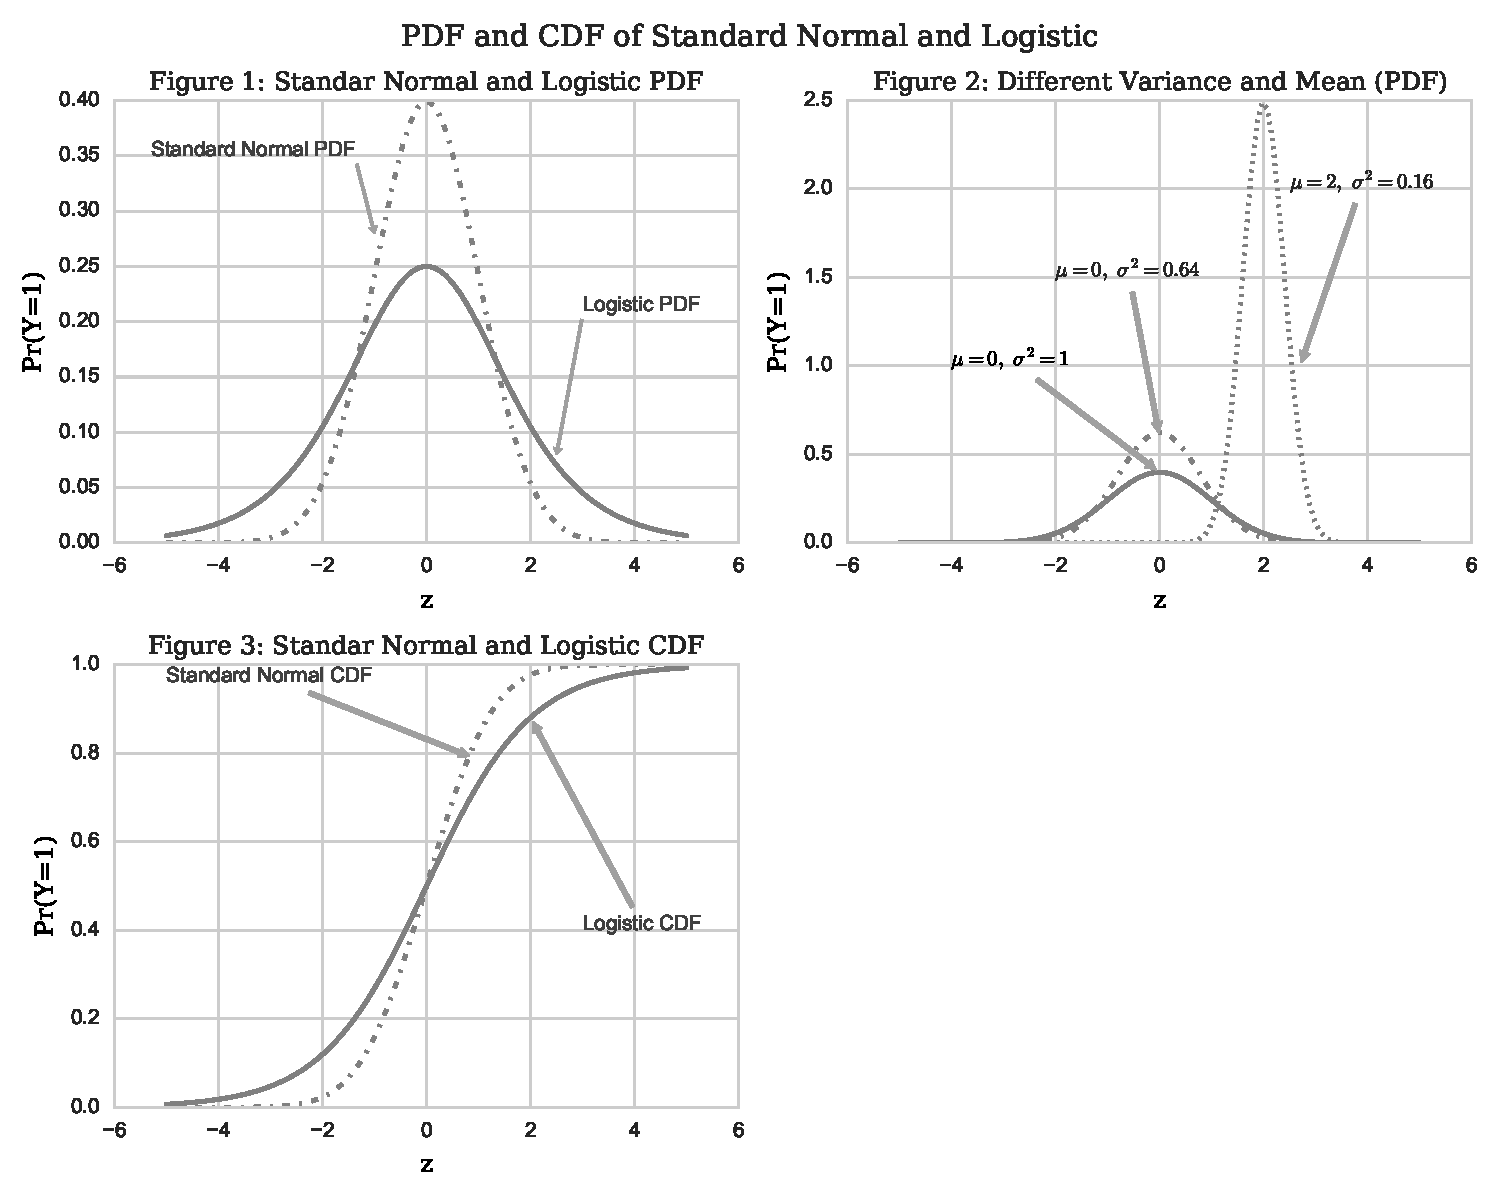
\includegraphics[width=1\textwidth]{Figure123.pdf}
\end{figure}

\FloatBarrier
\end{document}
